\documentclass{article}
\usepackage[utf8]{inputenc}
\usepackage{natbib}
\usepackage{graphicx}
\usepackage[brazil]{babel}

\title{IF866 - Criatividade Computacional}
\author{Matheus Victor Alves da Silva}
\date{\vspace{-5ex}}
\date{Dezembro 2021}

\begin{document}

\maketitle

\section{Introdução}
A disciplina de Criatividade Computacional do curso de Ciência da Computação do CIn-UFPE (Centro de Informática UFPE), ministrada pelo professor Filipe Calegario, abrange os processos e as interseções existentes entre os universos do design, da computação e da arte  \citep{SharePET}. Nessa disciplina, oferece-se aos alunos a possibilidade de aprender sobre assuntos como  Área de Criatividade Computacional, Teorias sobre Criatividade, Aplicações Artísticas e Mercado de NFTs. O principal dessa disciplina é o desenvolvimento de debates, mini projetos e projetos sobre os assuntos discutidos  \citep{Disciplina}.

\begin{figure}[h!]
\centering
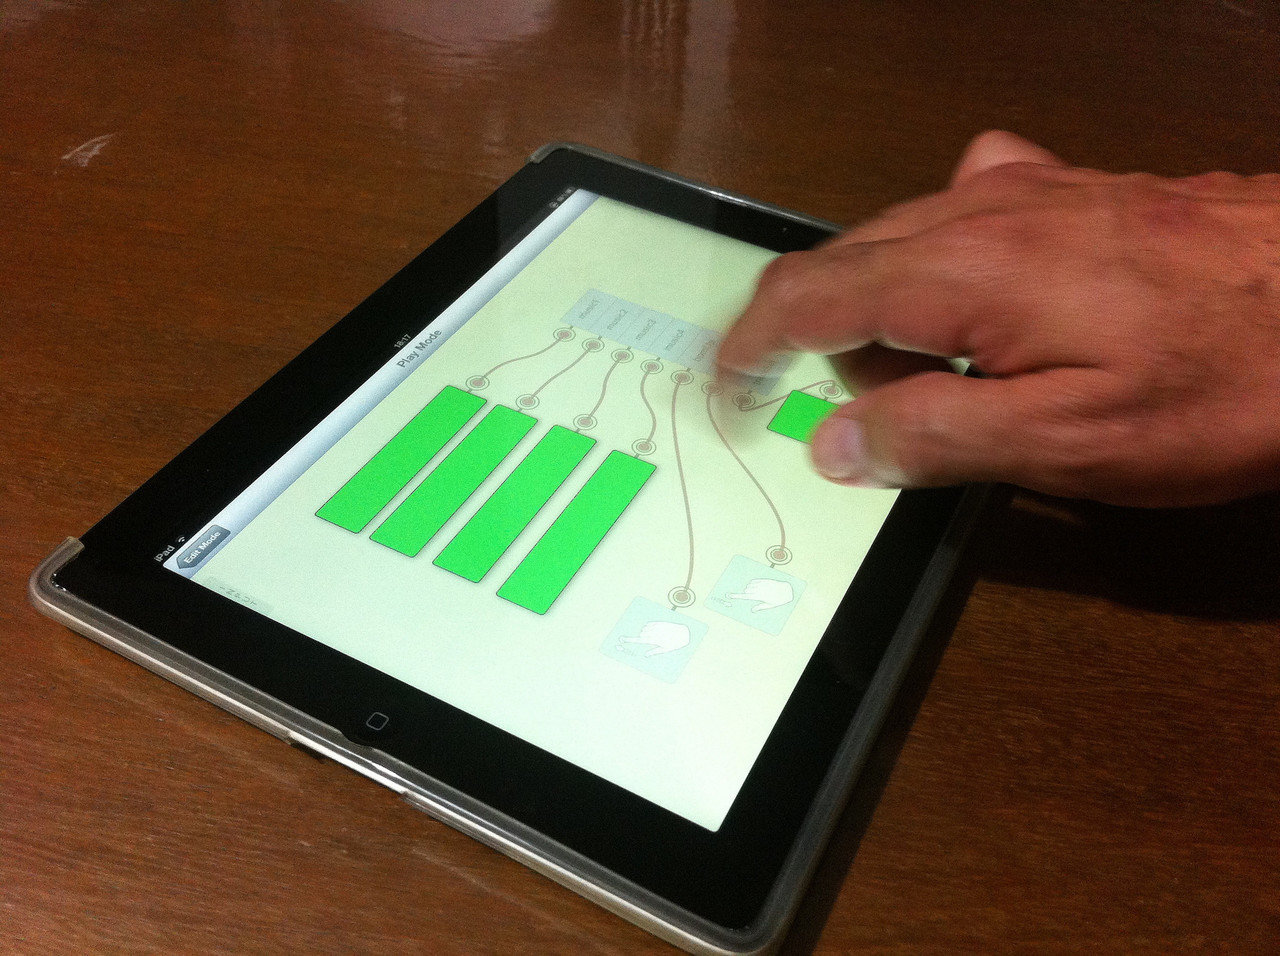
\includegraphics[scale=0.110]{CriatividadeComputacional.jpg}
\caption{Ferramenta para criar Arte  \citep{Imagem}}
\label{fig: CriatividadeComputacional.jpg}
\end{figure}

\section{Relevância}
Criatividade Computacional é uma disciplina eletiva para alunos que tenham interesse em Computação, Experimentação e Arte, sem necessariamente ter “habilidades” artísticas mas que procure por meios e técnicas para prototipar ferramentas para criar arte. Dessa forma, os conceitos aprendidos tem diversas aplicações no mundo artístico e com o possível avanço da Web3 com serviços que utilizam cada vez mais desse mundo Tokens, Criptomoedas e descentralização, o mercado de NFTs (Non-fungible token) se torna cada vez mais atraente para o mercado artístico digital. 

\section{Relação com outras disciplinas}
\begin{table}[h]
 \centering
 {\renewcommand\arraystretch{1.25}
 \caption{Relações}
 \begin{tabular}{ l l }
  \cline{1-1}\cline{2-2}  
    \multicolumn{1}{|p{3.850cm}|}{Disciplina \centering } &
    \multicolumn{1}{p{4.217cm}|}{Relação \centering }
  \\  
  \cline{1-1}\cline{2-2}  
    \multicolumn{1}{|p{3.850cm}|}{IF760: Tópicos Avançados em Mídias e Interação  \citep{IF760}} &
    \multicolumn{1}{p{4.217cm}|}{Human-Robot Interaction(HRI) e investigação do estado da arte na área de HRI.}
  \\  
  \cline{1-1}\cline{2-2}  
    \multicolumn{1}{|p{3.850cm}|}{IF702: Redes neurais  \citep{IF702}} &
    \multicolumn{1}{p{4.217cm}|}{{Fundamentos Matemáticos, Modelos de Aprendizagem, Redes Convolucionais e Deep Learning.}}
  \\ 
  \cline{1-1}\cline{2-2}  
    \multicolumn{1}{|p{3.850cm}|}{IF755: Realidade aumentada  \citep{IF755}} &
    \multicolumn{1}{p{4.217cm}|}{Aplicações de Realidade Aumentada.}
  \\ 
  \hline

 \end{tabular} }
\end{table}

\bibliographystyle{plain}
\bibliography{references}

\end{document}
